\documentclass[tikz,border=12pt]{standalone}
\usepackage{amsmath,amssymb}

\begin{document}
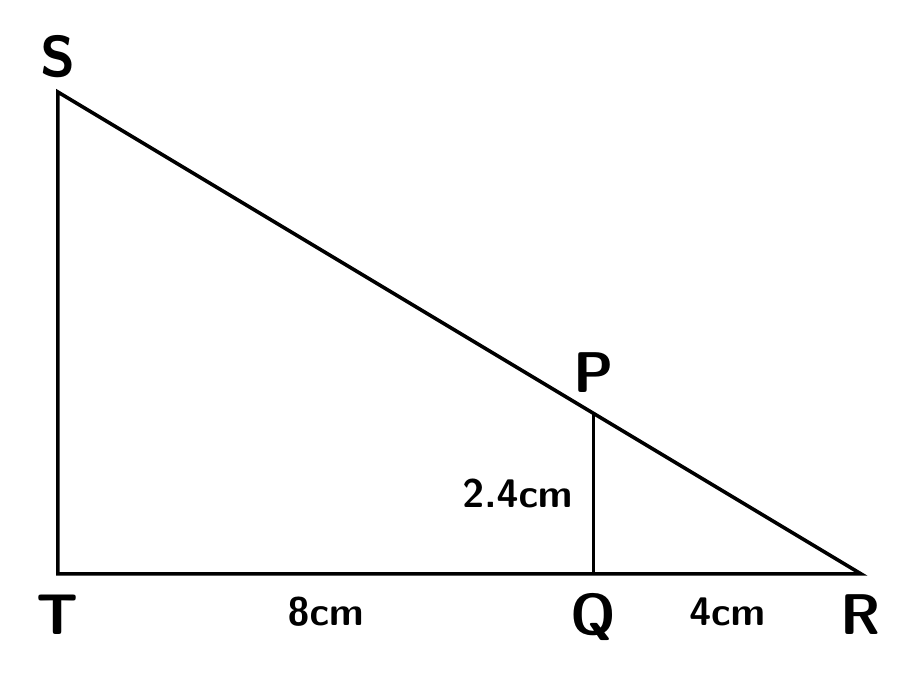
\begin{tikzpicture}[scale=0.85]
    % Coordinates (scaled for clean visual proportions)
    % Let TR = 12 cm, T at (0,0), Q at (8,0), R at (12,0)
    % Height ST = 7.2 cm, PQ = 2.4 cm
    \coordinate (T) at (0, 0);
    \coordinate (Q) at (8, 0);
    \coordinate (R) at (12, 0);
    \coordinate (S) at (0, 7.2);
    \coordinate (P) at (8, 2.4);
    
    % Draw large triangle STR
    \draw[line width=1.3pt] (T) -- (R) -- (S) -- cycle;
    
    % Draw vertical segment PQ
    \draw[line width=1.2pt] (P) -- (Q);
    
    % Vertices labels
    \node[above=2pt, font=\huge\sffamily\bfseries] at (S) {S};
    \node[below=4pt, font=\huge\sffamily\bfseries] at (T) {T};
    \node[above=4pt, font=\huge\sffamily\bfseries] at (P) {P};
    \node[below=4pt, font=\huge\sffamily\bfseries] at (Q) {Q};
    \node[below=4pt, font=\huge\sffamily\bfseries] at (R) {R};
    
    % Dimension labels
    \node[below=5pt, font=\Large\sffamily\bfseries] at (4.0, 0) {8cm};
    \node[below=5pt, font=\Large\sffamily\bfseries] at (10.0, 0) {4cm};
    \node[left=4pt, font=\Large\sffamily\bfseries] at (8.0, 1.2) {2.4cm};
    
\end{tikzpicture}
\end{document}
